\hypertarget{a00004}{
\section{Dokumentacja klasy md5wrapper}
\label{a00004}\index{md5wrapper@{md5wrapper}}
}
{\tt \#include $<$md5wrapper.h$>$}

Diagram współpracy dla md5wrapper:\nopagebreak
\begin{figure}[H]
\begin{center}
\leavevmode
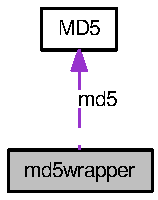
\includegraphics[width=112pt]{a00054}
\end{center}
\end{figure}
\subsection*{Metody publiczne}
\begin{CompactItemize}
\item 
\hyperlink{a00004_ae8138b76b89d93a4c21077b76d57c07}{md5wrapper} ()
\item 
\hyperlink{a00004_65e78258ad508d83be81d395f8bd43f4}{$\sim$md5wrapper} ()
\item 
std::string \hyperlink{a00004_225ba5a78228b867c3f17fdba959d8e6}{getHashFromString} (std::string text)
\item 
std::string \hyperlink{a00004_e6cd2a7928b997c5d6388ae81a0d841a}{getHashFromFile} (std::string filename)
\end{CompactItemize}


\subsection{Opis szczegółowy}


Definicja w linii 23 pliku md5wrapper.h.

\subsection{Dokumentacja konstruktora i destruktora}
\hypertarget{a00004_ae8138b76b89d93a4c21077b76d57c07}{
\index{md5wrapper@{md5wrapper}!md5wrapper@{md5wrapper}}
\index{md5wrapper@{md5wrapper}!md5wrapper@{md5wrapper}}
\subsubsection[{md5wrapper}]{\setlength{\rightskip}{0pt plus 5cm}md5wrapper::md5wrapper ()}}
\label{a00004_ae8138b76b89d93a4c21077b76d57c07}




Definicja w linii 70 pliku md5wrapper.cpp.\hypertarget{a00004_65e78258ad508d83be81d395f8bd43f4}{
\index{md5wrapper@{md5wrapper}!$\sim$md5wrapper@{$\sim$md5wrapper}}
\index{$\sim$md5wrapper@{$\sim$md5wrapper}!md5wrapper@{md5wrapper}}
\subsubsection[{$\sim$md5wrapper}]{\setlength{\rightskip}{0pt plus 5cm}md5wrapper::$\sim$md5wrapper ()}}
\label{a00004_65e78258ad508d83be81d395f8bd43f4}




Definicja w linii 77 pliku md5wrapper.cpp.

\subsection{Dokumentacja funkcji składowych}
\hypertarget{a00004_e6cd2a7928b997c5d6388ae81a0d841a}{
\index{md5wrapper@{md5wrapper}!getHashFromFile@{getHashFromFile}}
\index{getHashFromFile@{getHashFromFile}!md5wrapper@{md5wrapper}}
\subsubsection[{getHashFromFile}]{\setlength{\rightskip}{0pt plus 5cm}std::string md5wrapper::getHashFromFile (std::string {\em filename})}}
\label{a00004_e6cd2a7928b997c5d6388ae81a0d841a}




Definicja w linii 100 pliku md5wrapper.cpp.

Oto graf wywołań dla tej funkcji:\nopagebreak
\begin{figure}[H]
\begin{center}
\leavevmode
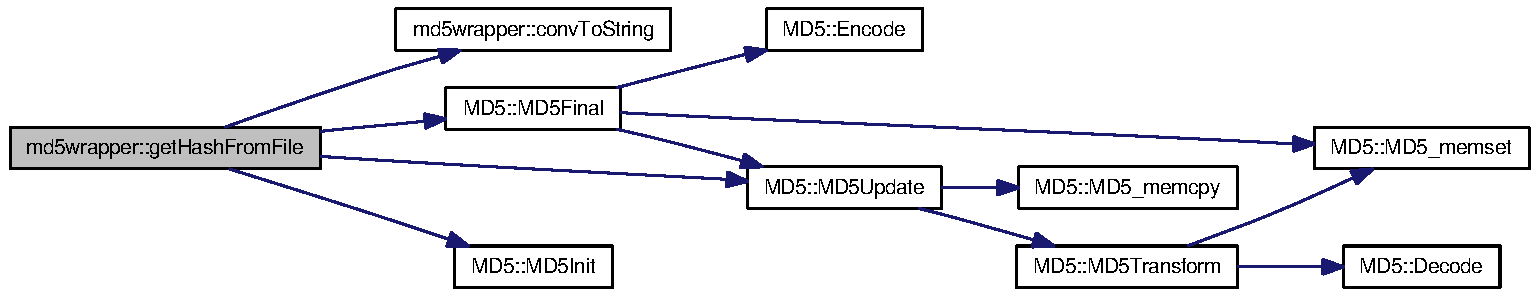
\includegraphics[width=222pt]{a00004_e6cd2a7928b997c5d6388ae81a0d841a_cgraph}
\end{center}
\end{figure}
\hypertarget{a00004_225ba5a78228b867c3f17fdba959d8e6}{
\index{md5wrapper@{md5wrapper}!getHashFromString@{getHashFromString}}
\index{getHashFromString@{getHashFromString}!md5wrapper@{md5wrapper}}
\subsubsection[{getHashFromString}]{\setlength{\rightskip}{0pt plus 5cm}std::string md5wrapper::getHashFromString (std::string {\em text})}}
\label{a00004_225ba5a78228b867c3f17fdba959d8e6}




Definicja w linii 87 pliku md5wrapper.cpp.

Dokumentacja dla tej klasy została wygenerowana z plików:\begin{CompactItemize}
\item 
/home/pawel/Dokumenty/Uczelnia/grupappz/Source/Ass8-server/include/md5/\hyperlink{a00012}{md5wrapper.h}\item 
/home/pawel/Dokumenty/Uczelnia/grupappz/Source/Ass8-server/include/md5/\hyperlink{a00011}{md5wrapper.cpp}\end{CompactItemize}
